\documentclass[12pt]{exam}
\usepackage{amsthm}
\usepackage{libertine}
\usepackage[utf8]{inputenc}
\usepackage[margin=1in]{geometry}
\usepackage{amsmath,amssymb}
\usepackage{multicol}
\usepackage[shortlabels]{enumitem}
\usepackage{siunitx}
\usepackage{cancel}
\usepackage{graphicx}
\usepackage{pgfplots}
\usepackage{listings}
\usepackage{tikz}


\pgfplotsset{width=10cm,compat=1.9}
\usepgfplotslibrary{external}
\tikzexternalize

\newcommand{\class}{Termodinamica} % This is the name of the course 
\newcommand{\examnum}{Taller 1} % This is the name of the assignment
\newcommand{\examdate}{12/02/2023} % This is the due date
\newcommand{\timelimit}{}





\begin{document}
\pagestyle{plain}
\thispagestyle{empty}

\noindent
\begin{tabular*}{\textwidth}{l @{\extracolsep{\fill}} r @{\extracolsep{6pt}} l}
	\textbf{\class} & \textbf{Name:} & \textit{Sergio Montoya Ramirez}\\ %Your name here instead, obviously 
\textbf{\examnum} &&\\
\textbf{\examdate} &&\\
\end{tabular*}\\
\rule[2ex]{\textwidth}{2pt}
% ---



\section{Capitulo 1.3}
\begin{enumerate} %You can make lists!

	\item Un decimo de kilogramo de NaCl y 0.15 kg de azucar son disueltos en 0.5 kg de agua pura. El volumen resultante del sistema termodinamico es $0.55\times10^{-3}m^3$.
		\begin{enumerate}
			\item Primero debemos pasar los valores que nos dieron a gramos
				\begin{itemize}
					\item 100 g de NaCl
					\item 150 g de $C_{12}H_{22}O_{11}$
					\item 500 g de $H_2O$
				\end{itemize}
			\item Cuales son los numeros molares de cada componenete.
				Para esto lo primero que tenemos que hacer es utilizar una tabla periodica. En este caso vamos a utilizar ptable.com sin embargo para tener mayor facilidad aproximaremos los valores al entero mas cercano.
				\begin{enumerate}
					\item $NaCl$
						\begin{eqnarray*}
							Na: & 23\times 1 =&23\\
							Cl: & 35\times 1 =&35\\
							&Total =&58
						\end{eqnarray*}
					\item $C_{12}H_{22}O_{11}$
						\begin{eqnarray*}
							C:&12\times 12=&144\\
							H:&1\times 22=&22\\
							O:&16\times 11=&176\\
							& Total =& 342
						\end{eqnarray*}
					\item $H_2O$
						\begin{eqnarray*}
							H: & 1\times 2= & 2\\
							O: & 16\times 1= & 16\\
							& Total = & 18
						\end{eqnarray*}
				\end{enumerate}
			\item Ahora vamos a encontrar el numero de moles que tiene cada compuesto
				\begin{enumerate}
					\item $NaCl$
						\begin{align*}
							& 100 g/58 \frac{g}{mol} = 1.72
						\end{align*}
					\item $C_{12}H_{22}O_{11}$
						\begin{align*}
							& 150/342 = 0.43
						\end{align*}
					\item $H_2O$
						\begin{align*}
							& 550/18 = 27.77
						\end{align*}
					\item Total
						\begin{align*}
							& 27.77 + 1.72 + 0.43 = 29.92
						\end{align*}
				\end{enumerate}
			\item Cuales son las fracciones molares
				\begin{enumerate}
					\item $NaCl$
						\begin{align*}
							& 1.72/29.92 = 0.057
						\end{align*}
					\item $C_{12}H_{22}O_{11}$
						\begin{align*}
							& 0.43/29.92 = 0.014
						\end{align*}
					\item $H_2O$
						\begin{align*}
							& 27.77/29.92 = 0.928
						\end{align*}
				\end{enumerate}
			\item calcular el volumen molar
				Dado el volumen que nos dieron y con los moles que ya calculamos podemos calcular facilmente lo que nos piedieron.
				\begin{align*}
					\frac{0.55\times10^{-3}}{29.9}=18\times^{-6} \frac{m^3}{mol}
				\end{align*}
		\end{enumerate}
	\item Naturalmente el Boron tiene una masa atomica de 10.811 g. Es una mezcla de Isotopos $^{10}B$ con una masa atomica de 10.0129 g y $^{11}B$ con una masa atomica de 11.0093. Cual es la fracción molar de $^{10}B$ en la mixtura.
		Por la definicion de fraccion molar tenemos que 
		\begin{align*}
			&A(M_{^{10}B}) + B(M_{^{11}B}) = M_{Boron}\\
			&A + B = 1\\
			&B = 1-A\\
			&A(10.0129) + (1-A)(11.0093) = 10.811\\
			&A(10.0129-11.0093) = 10.811-11.0093\\
			&A(-0.9964) = -0.1983\\
			&A = \frac{0.1983}{0.9964}\\
			&A = 0.1990\\
		\end{align*}
		Por lo tanto, el valor de A (que es la fracción molar de $^{10}B$) es 0.1990
	\item Una solución de Azucar en agua es $20\%$ azucar por peso. Cual es la fracción molar del azucar en esa solución?

		Sea $M$ la masa total del compuesto por lo tanto sabemos que
		\begin{align*}
			0.2M + 0.8M = M\\
		\end{align*}
		En el punto uno calculamos cual es el numero molar del Agua y del Azucar por lo que reutilizaremos estos valores para no tener que recalcularlos.
		\begin{align*}
			&N_{azucar} = \frac{0.2M}{342} = 0.000588M\\
			&N_{agua} = \frac{0.8M}{18}=0.0444\\
			&X_{azucar} = \frac{0.000588M}{0.044M+0.000588M}\\
			&X_{azucar} = 0.0128
		\end{align*}
\end{enumerate}
\vspace{15cm}
\section{Capitulo 1.8}
\begin{enumerate}
	\item Para un sistema gaseoso particular a sido determinado que la energia esta dado por $$U = 2.5PV + C$$ donde C es una constante. Este sistema es inicialmente en el estado $P = 0.2 MPa$, $V=0.01 m^3$ Este fue designado como punto A en la figura \ref{fig:Imagen183}. El sistema es tomado por un ciclo de tres procesos como se muestra en la figura \ref{fig:Imagen183}. Calcule Q y W para cada uno de estos tres proceso. Calcule Q y W para el proceso $A\to B$ por medio de la parabola $P=10^5 + 10^9 \times (V - .02)^2$
		\begin{figure}[h]
			\centering
			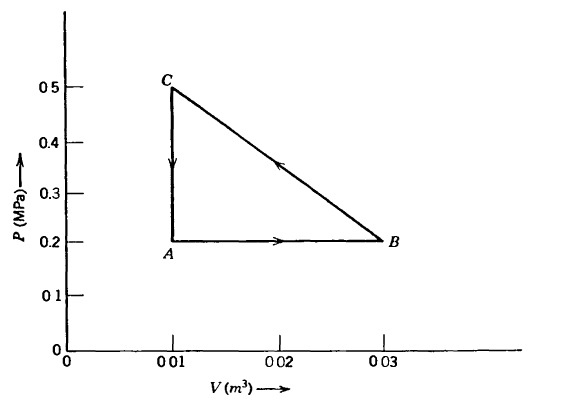
\includegraphics[scale=0.5]{Imagen183.jpeg}
			\caption{Grafica del problema 1-8.3 en esta aparecen todos los puntos dados en el enunciado. Recuperado del libro Callen}
			\label{fig:Imagen183}
		\end{figure}
		
		Primero tomemos los datos que tenemos por la grafica y la descripción.
		\begin{table}[h]
			\centering
			\caption{Datos que tenemos previo a la realización del ejercició. Estos fueron adquiridos de la descripción y la grafica \ref{fig:Imagen183}}
			\label{table:Datos}
			\begin{tabular}{|c|c|c|c|}
				\hline
				$V_A$ & 0.01 & $P_A$ & $2\times 10^5$ \\
				$V_B$ & 0.03 & $P_B$ & $2\times 10^5$ \\
				$V_C$ & 0.01 & $P_C$ & $5\times 10^5$ \\
				\hline
			\end{tabular}
		\end{table}

		Una vez tenemos esto, note que
		\begin{align*}
			& W_{CA} = 0\\
			& W_{AB} = -(V_B - V_A)\cdot P_A = -(0.03 - 0.01)\cdot 2\times 10^5 = -4000 J\\
			& W_T = (P_C - P_A)\cdot (V_B - V_A)\cdot\frac{1}{2}\\
			& W_T = (0.5-0.2)MPa\cdot(0.03-0.01)m^3\frac{1}{2} = 3000J
		\end{align*}
		Una vez teniendo esto podemos tomar que $W_T = W_{AB} + W_{BC} + W_{CA}$ y ya tenemos dos de tres valores en los puntos anteriores.
		\begin{align*}
			& W_T = W_{AB} + W_{BC} + W_{CA}\\
			& W_BC = W_T - W_{AB} - W_{CA}\\
			& W_BC = 3000 + 4000 + 0 = 7000
		\end{align*}

		Por otra parte, para el siguiente punto utilizaremos las siguientes ecuaciones
		\begin{align}
			& Q_{total} = - W_{total} \label{eq:Igual}\\
			& Q_{total} = Q_{AB} + Q_{BC} + Q_{CA}\label{eq:QTotal}\\
			& U =2.5 PV + \textit{Const \label{eq:Estado}}\\
			& \Delta U = U_F - U_0 \label{eq:DeltaU}\\
			& \Delta U = Q + W \label{eq:Normal}
		\end{align}
		Esto nos resulta util pues podemos encontrar $Q$ desde la ecuación \ref{eq:Normal} con el siguiente despeje
		\begin{align*}
			& \Delta U = Q + W\\
			& Q = \Delta U - W\\
		\end{align*}

		Esto es util puesto que, para cada trayecto tenemos su trabajo (Lo calculamos justo antes de lo aqui expuesto) y ademas podemos encontrar $\Delta U$ facilmente con la ecuación \ref{eq:DeltaU} pues podemos encontrar los valores de cada punto con la ecuación \ref{eq:Estado} dado que sabemos la presion y el volumen como se muestra en la tabla \ref{table:Datos}.

		Ya con todo esto podemos resolver la ecuación con
		\begin{align*}
			Q &= (U_F - U_0) - W\\
			Q &= (2.5 P_FV_F - 2.5 P_0V_0) - W\\
			Q &= 2.5(P_FV_F -P_0V_0) - W
		\end{align*}
		Una vez que tenemos eso lo unico que falta es reemplazar los datos. con los que ya tenemos y eso nos quedaria
		\begin{align*}
			Q_{AB} &= 2.5(2\times 10^5\cdot 0.03-2\times 10^5 \cdot 0.01)-(-4000) = 14000\\
			Q_{BC} &= 2.5(5\times 10^5\cdot 0.01-2\times 10^5 \cdot 0.03)-7000 = -9500\\
			Q_{CA} &= 2.5(2\times 10^5\cdot 0.01-5\times 10^5 \cdot 0.01)-0 = -7500
		\end{align*}

		Ahora bien, para verificar que lo aqui hallado es correcto, confirmemos la ecuación \ref{eq:Igual} utilizando la ecuación \ref{eq:QTotal}.
		\begin{align*}
			Q_{total} &= -W_{total}\\
			Q_{AB} + Q_{BC} + Q_{CA} &= -W_{total}\\
			14000 - 9500 - 7500 &= -W_{total}\\
			-3000 &= -3000\ 
		\end{align*}

		Hasta aqui era la primera parte del problema. Sin embargo, el libro tambien nos pide que encontremo $Q$ y $W$ para un proceso que va de $A$ a $B$ por un proceso que va por la parabola $P = 10^5 + 10^9 \times (V-0.02)^2$

		Para resolver esto, primero iniciemos notando que $\Delta U$ es independiente de la trayectoria y sabemos por \ref{eq:DeltaU} como calcularlo que en este caso nos da $10000$. Ahora bien, con la ecuación \ref{eq:DeltaU} podemos calcular $Q$ como lo mostramos previamente. Para esto nos hace falta $W$ que es por definición $$W=-\int PdV$$

		por lo tanto, para hallar $W$ debemos hacer:
		\begin{align*}
			W = -\int PdV &= -\int_{0.01}^{0.03}10^5 + 10^9 \times (V-0.02)^2\\
			W &= -\int_{0.01}^{0.03} 10^5 + 10^9 \times (v^2 - 0.04V + 4\times 10^{-4}) dV\\
			W &= -\int_{0.01}^{0.03} 10^5 + 10^9 v^2 -4\times 10^7 v + 4\times 10^5 dV\\
			W &= -\int_{0.01}^{0.03} 10^9 v^2 + 4\times 10^7 v + 5\times 10^5 dV\\
			W &= -\left(\frac{10^9v^3}{3} + \frac{4\times 10^7v^2}{2} + 5\times 10^5v\right)|_{0.01}^{0.03}\\
			W &= -(6000-3333.3) = -2666.6
		\end{align*}
		Una vez tenemos esto, solo nos  queda reemplazar, como habiamos dicho previamente, en la ecuación \ref{eq:DeltaU}. lo que nos deja con
		\begin{align*}
			&Q = \delta U - W\\
			&Q = 10000 - (-2666.6)\\
			&Q = 12666.6
		\end{align*}
		Y con esto acabamos este punto.
	\item Para el sistema del problema 1.8-3 encuentre la ecuación de los adiabatas en el plano P-V. (Es decir, encuentre la forma de la curva P=P(V) tal que dQ = 0)
		
		Dado que nos dan para este sistema particular la siguiente ecuación partamos de ella.
		\begin{align*}
			& U = 2.5PV + constant\\
			& dU = 2.5PdV + 2.5VdP
		\end{align*}
		por otro lado sabemos que la primera ley de la termodinamica para un adiavatico es
		$\Delta U = W$
		Lo cual en nuestro caso tendriamos lo siguiente:
		$$\Delta U = -P dV$$
		con esto podemos igualar ambos y nos quedaria
		\begin{align*}
			& dU = 2.5PdV + 2.5VdP = -PdV\\
			& = 2.5PdV + 2.5VdP + PdV = 0\\
			& = 3.5PdV + 2.5VdP = 0\\
			& \text{Multiplicamos por 2 para quitarnos los decimales}\\
			& = 7PdV + 5VdP = 0\\
			& \text{Ahora dividimos tanto por T como por V en ambos lados}\\ 
			& \text{para que las variables queden con sus diferenciales}\\
			& = \frac{7\cancel{P}dV}{\cancel{P}} + \frac{5Vdp}{P} = \frac{0}{P}\\
			& = 7\frac{dv}{V} + 5\frac{\cancel{V}dP}{P\cancel{V}} = \frac{0}{V}\\
			& = 7\frac{dv}{V} + 5\frac{dP}{P} = 0\\
			& \text{Ahora integremos}\\
			& = \int 7\frac{dV}{V} + 5\frac{dP}{P} =  0\\
			& = 7 \int \frac{dV}{V} + 5 \int \frac{dP}{P} = \\
			& = 7 \ln(\frac{P}{constante}) + 5 \ln(\frac{V}{constante_2}) = 0\\
			& = P^7V^5 = constante\\
		\end{align*}
		\vspace{5cm}
	\item Dos moles de un sistema particular se encuentra que la formula de la energia interna es 
		$$U = APV^2$$
		Donde A y P son extensivas y V, U , N son intensivas. 

		Para solucionar este punto debemos encontrar una manera de ingresar N que cumpla que al duplicar su valor tambien se duplique V y U.

		Por lo tanto podemos saber que N debe estar ahi y para considerar las posibles inserciones asumamos que este esta elevado a un valor y multiplicado por otro.
		\begin{align*}
			& U = XN^yAPV^2\\
			& U = X2^{y}APV^2 = APV^2\\
			& 2U = X4^{y}AP(2V)^2 = 2APV\\
			& 2U = X4^{y}AP4V^{2}\\
			& y = -1\\
			& 2U = X\frac{1}{\cancel{4}}AP\cancel{4}V^2\\
			& X = 2\\
			& 2U = 2APV^2\\
			& \text{Con los mismos datos tenemos}\\
			& U = \frac{2}{N}APV^2\\
			& U = \frac{2}{2}APV^2 = APV^2 ; N= 2\\
		\end{align*}
		Se hace con estos valores pues esta es la información que se nos da.
		\end{enumerate}

\section*{B. Parte Escrita}

Quizas uno de los logros mas grandes de la física es la conservación de la energia. Este no fue fruto de una noche de sorprendente inspiración si no el trabajo de muchas de esas noches que cada vez iban aportando al concepto que tenemos hoy en dia. Uno de esos grandes cambios que tuvo el principio de conservación de la energia fue cuando se describio la energia calorifica. Esta adición fue especialmente potente pues permitio salvar la conservación hasta en los momentos mas extremos (Como lo seria la bomba atomica). Sin embargo, aun con sus profundas implicaciones y consecuencias la energia calorifica tuvo un viaje rockanbolezco. Este inicio y fue desarrollado, mayoritariamente, por puros efectos macroscopicos y logro su aceptación antes de que los atomos fueran aceptados. Este viaje inicio con C. Rumford y acabo con James Joule describiendo (de manera muy similar a la moderna) el concepto de calor que tenemos hoy en dia.

Ahora bien, uno de los problemas que tiene estudiar la energia es que la manera en la que se mide. Esto pues no es una "medida clasica" si es que este concepto siquiera existe. Me explico, la energia, por lo general, no tiene efectos macroscopicos como la altura, la velocidad o la masa. Aun así, note que todos estos tienen participación en la energia. Asi, la mayoria de energias tienen un efecto o componentes macroscopicos facilmente reconocibles. Sin embargo, la energia calorifica es especialmente dificil pues esta no tiene aquellas caracterizticas de las que hablamos. Pero entonces, ¿Como medimos el calor?. Para esto hay varios temas que nos interesan. 

Primero, nos interesa separar el sistema y hacer que los efectos del medio sea menor, de modo tal que sepamos que la energia se conserva. En concepto es sencillo lo que hace, aun asi, este fue un gran logro del ingenio de experimentales. Aquellas cosas que nos permiten separar el sistema fueron conocidas como paredes adiabaticas.

Segundo, nos incumbe hacer la aclaración de que no es la energia lo que deseamos medir o lo que tiene valor, si no la diferencia de energia la que nos interesa. Entonces para eso utilizamos paredes adiabaticas y un sistema experimental que nos permitira transformar la energia en trabajo y calcular por medio de cinematica y dinamica la energia que nos interesa.

Sin embargo, todo esto nos permite poner un sistema en una condición inicial arbitraria. Sin embargo, esto no tiene por que ser asi. Las observaciones de James Joule nos permiten identificar que dos estados acoplados (es decir que sus energias tienen efectos entre si) pueden cambiar de energia interna y como tal asi definio el calor. Las particularidades de este y los detalles que presentan se escapan de las capacidades del texto. Pero con eso Joule mostro que la energia puede ser medida.
\end{document}
